\subsection{Pole-zero compensation di una sonda}

\begin{wrapfigure}[11]{r}{0.45\textwidth}
\centering
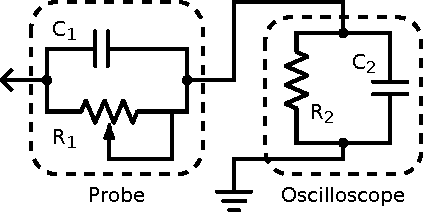
\includegraphics[width=.35\textwidth]{../E08/latex/probe.pdf}
\caption{Schema del circuito di misura composto dall'oscilloscopio e dalla sonda.}
\label{cir8:probe}
\end{wrapfigure}

La \textit{pole-zero compensation} è una tecnica che permette di compensare dei poli del sistema. Tale procedimento ci permette di eliminare dipendenze dalla grequenza e di effettuare misure precise di circuiti senza interferenze da parte dell'apparato di misura.
%L'alta impedenza determina una forte dipendenza dalla frequenza generata ad esempio da grandi resistenze, in quanto subentrano induttanze parassite, oppure direttamente da piccole capacità.

Essa consiste nel posizionare, aggiungendo un'ulteriore parte circuitale, uno zero alla funzione di trasferimento esattamente nel punto in cui esiste un polo .
In equazioni si traduce con:

\[
  \begin{array}{lr}
H(s) = \frac{a(s)}{b(s)} \quad tc \quad b(s_0) = 0 \\
f(s) \quad tc \quad f(s_0) = 0
  \end{array}\left\}
\quad \longrightarrow \quad H'(s) = \frac{a(s)f(s)}{b(s)} \quad tc \quad H'(s_0) = 0
\right.
\]

Per ottenere questo risultato, si antepone all'oscilloscopio una sonda compensata il cui circuito schematizzato è proposto in Figura \ref{cir8:probe}.
Come si può notare la sonda e l'oscilloscopio formano un partitore e pertanto la tensione misurata dallo strumento non sarà la stessa del circuito.
Sarà determinata dalla funzione di trasferimento:

\begin{equation}
H(s)=\frac{Z_{osc}}{Z_{probe}+Z_{osc}} = \frac{R_2}{R_1+R_2}\,\frac{1+R_1C_1s}{1+\frac{R_1R_2}{R_1+R_2}(C_1+C_2)s}
\end{equation}

Da questa formula è evidente che la compensazione del polo sia ha quando la seconda frazione è uguale ad \num{1} e quindi il partitore diventa completamente resistivo:
\begin{equation*}
1+R_1C_1s = 1+\frac{R_1R_2}{R_1+R_2}(C_1+C_2)s
\end{equation*}
da cui
\begin{equation}
R_1 = R_2 \frac{C_2}{C_1}
\end{equation}

Questa relazione permette di spostare lo zero della sonda proprio sul polo dell'oscilloscopio permettendone la compensazione.
Dal punto di vista pratico, rendiamo la sonda insensibile alla frequenza e, fissati i parametri $R_2$, $C_2$ e $C_1$, si varia $R_1$ finché l'oscilloscopio non misura la stessa tensione $V_{in}$ ridotta di un fattore $\frac{R_2}{R_1+R_2}$.



\begin{figure}[htpc]
\centering
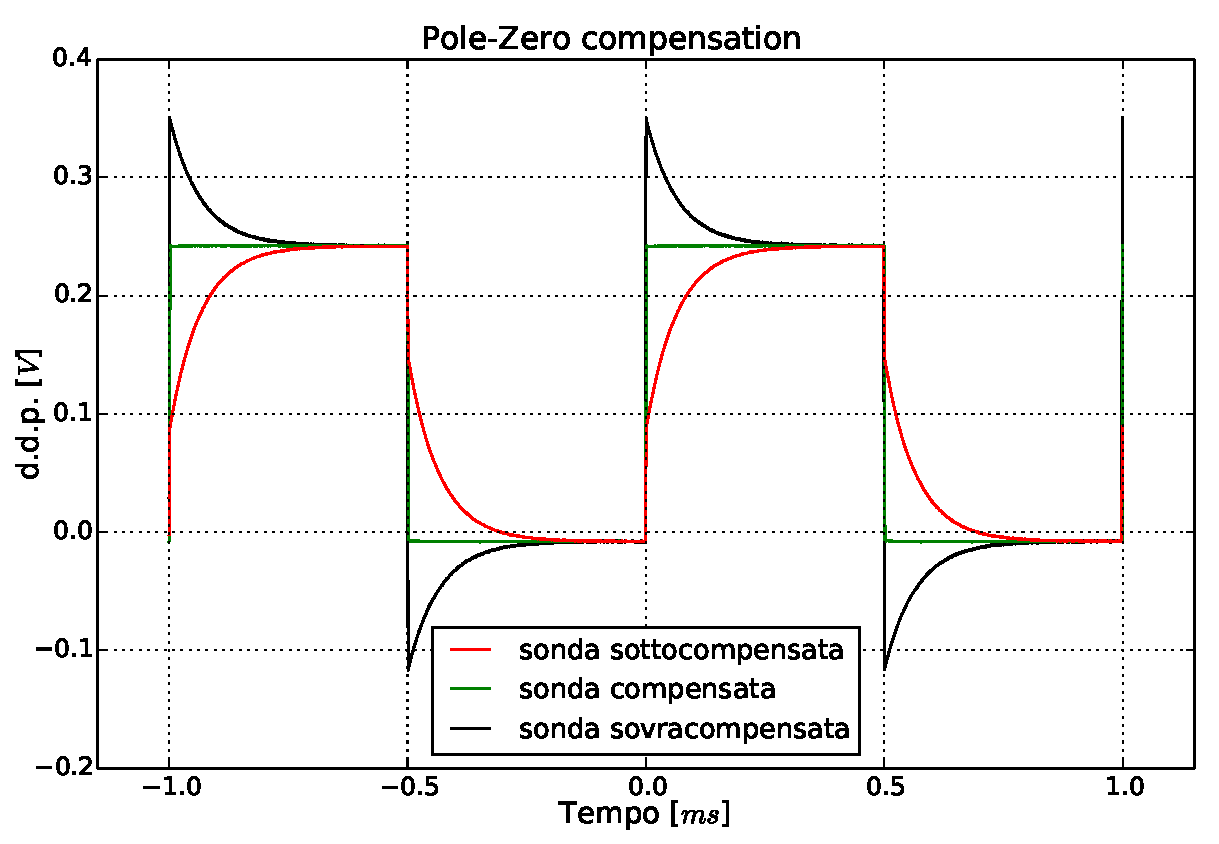
\includegraphics[width=.65\textwidth]{../E08/latex/compensation.pdf}
\caption{Risposta del circuito composto dalla sonda e dall'oscilloscopio visto dall'oscilloscopio stesso. La sonda è stata eccitata con un'onda quadra tramite il generatore interno dell'oscilloscopio.}
\label{fig8:compensation}
\end{figure}
